\documentclass[12pt,a4paper]{article}
\usepackage{geometry}
\geometry{left=2.5cm,right=2.5cm,top=2.0cm,bottom=2.5cm}
\usepackage[english]{babel}
\usepackage{amsmath,amsthm}
\usepackage{amsfonts}
\usepackage[longend,ruled,linesnumbered]{algorithm2e}
\usepackage{fancyhdr}
\usepackage{ctex}
\usepackage{array}
\usepackage{listings}
\usepackage{color}
\usepackage{graphicx}
\graphicspath{{hw10/figures/}{figures/}}
\lstset{
  basicstyle=\ttfamily\small,
  breaklines=true,
  columns=fullflexible,
  keepspaces=true,
  showstringspaces=false
}

\begin{document}


\title{
{《优化理论与算法》第10次作业
}
}
\date{}

 \author{
 姓名：\underline{焦传斌}~~~~~~
 学号：\underline{2024111223}~~~~~~}

\maketitle
\begin{itemize}
	\item 作业截止于{\bf 周日（5/17/2025）}，在Canvas系统中提交PDF或照片文件
	\item 作业题目的tex文件可以在Canvas中下载
	\item 鼓励相互讨论，但不要抄袭.
\end{itemize}
%%%%%%%%%%%%%%%%%%%%%%%%%%%%%%%%%%%%%%%%%%%%%%%%%%%%%%%%%%%%%%%%%
%%%%%%%%%%%%%%%%%%%%%%%%%%%%%%%%%%%%%%%%%%%%%%%%%%%%%%%%%%%%%%%%%

\section{阅读与积累}
\paragraph{1.1}
\begin{itemize}
	\item 复习 Boyd and Vandenberghe，也就是 Convex Optimization 教材，章节9.1，9.3相关
\end{itemize}

\section{迭代算法}

\paragraph{2.1} 假设$e(x^k)$ 是算法第$k$次迭代点 $x^k$的误差。下列误差的迭代复杂度（写成大O形式）与收敛速率分别是什么？
\begin{enumerate}
	\item[(a)] $e(x_k)=1/4^{\lfloor k/2 \rfloor}$
	\item[(b)] $e(x_k)=\sqrt{5}/2^{2^{k}}$
	\item[(c)] $e(x_k)=100/k$
	\item[(d)] $e(x_k)=\begin{cases}
	\frac{1}{k^2} & \quad \text{if } k \leq 50  \\  0.895^k & \quad \text{if } k>50 
	\end{cases}$
\end{enumerate}
利用Python或Matlab画图，类似课件P15页，将4种误差画在同一个图里面，要求一张图的坐标轴采用正常比例尺，另一张图的$y$轴采用semilogy的方式作图。

\textbf{解：}
记达到精度 $e(x^k)\leq \epsilon$ 所需的最小迭代次数为 $N(\epsilon)$。下面同时给出误差本身的收敛速率 $e_k=O(\cdot)$ 和迭代复杂度 $N(\epsilon)$。
\begin{itemize}
  \item[(a)] 因为
  \[
    e(x^k)=4^{-\lfloor k/2\rfloor},
  \]
  且 $\lfloor k/2\rfloor\geq k/2-1$，所以
  \[
    e(x^k)\leq 4\cdot 2^{-k}.
  \]
  因此收敛速率为
  \[
    e_k=O(2^{-k})=O\left(\left(\frac12\right)^k\right),
  \]
  即 R-线性收敛。另一方面，要达到 $e(x^k)\leq\epsilon$，只需
  \[
    \lfloor k/2\rfloor\geq \log_4(1/\epsilon).
  \]
  因此
  \[
    N(\epsilon)=O(\log(1/\epsilon)).
  \]

  \item[(b)] 有
  \[
    e(x^{k+1})
    =\frac{\sqrt5}{2^{2^{k+1}}}
    =\frac{1}{\sqrt5}\left(e(x^k)\right)^2.
  \]
  因此它是二阶收敛，误差收敛速率为
  \[
    e_k=O(2^{-2^k})=O\left(\frac{1}{2^{2^k}}\right).
  \]
  由
  \[
    \frac{\sqrt5}{2^{2^k}}\leq \epsilon
  \]
  得
  \[
    2^k\geq \log_2(\sqrt5/\epsilon),
    \qquad
    N(\epsilon)=O(\log\log(1/\epsilon)).
  \]

  \item[(c)] 由 $100/k\leq\epsilon$ 得
  \[
    N(\epsilon)=\left\lceil\frac{100}{\epsilon}\right\rceil
    =O(1/\epsilon).
  \]
  误差收敛速率为
  \[
    e_k=O(1/k),
  \]
  即次线性收敛。

  \item[(d)] 前 $50$ 步满足 $e(x^k)=1/k^2$，属于 $O(1/k^2)$ 的次线性下降；当 $k>50$ 时，
  \[
    e(x^k)=0.895^k.
  \]
  因而渐近误差收敛速率为
  \[
    e_k=O(0.895^k),
  \]
  是线性收敛，收敛因子为 $0.895$。对足够小的 $\epsilon$，
  \[
    k\geq \frac{\log(1/\epsilon)}{\log(1/0.895)},
    \qquad
    N(\epsilon)=O(\log(1/\epsilon)).
  \]
\end{itemize}


四种误差曲线如下。正常比例尺下 $100/k$ 数值较大，会压低其他曲线；semilogy 图更能看出不同收敛速率的差别。

\begin{center}
  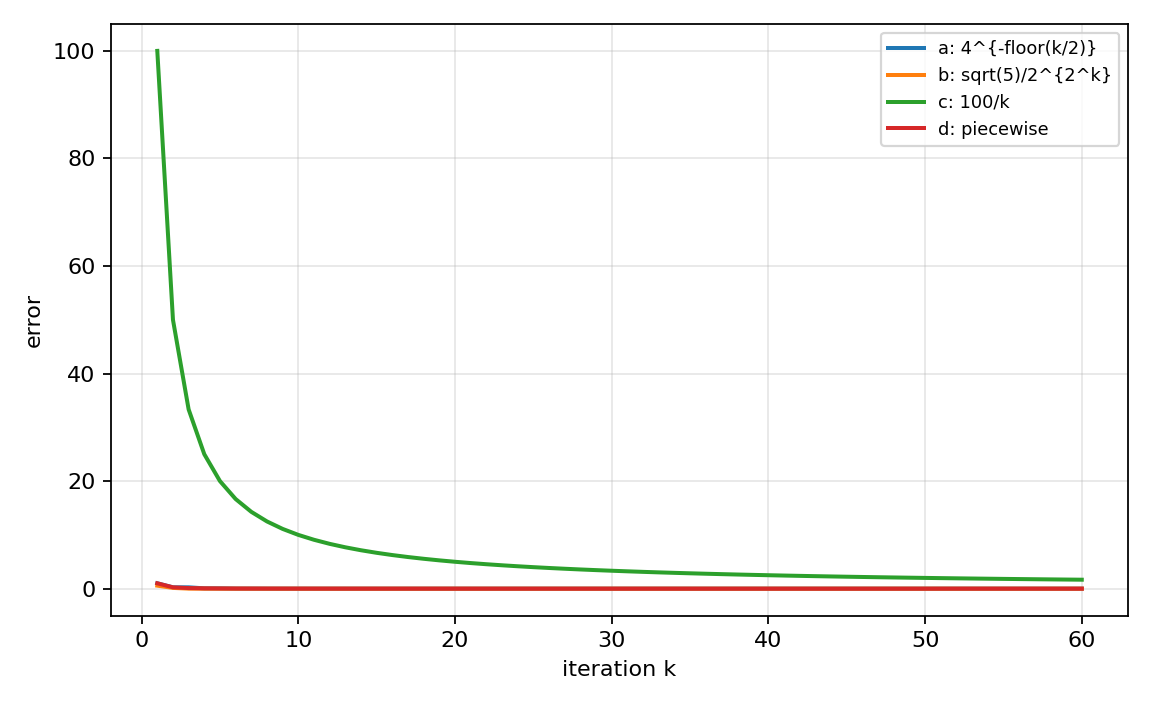
\includegraphics[width=0.78\textwidth]{hw10_2_1_linear.png}
\end{center}

\begin{center}
  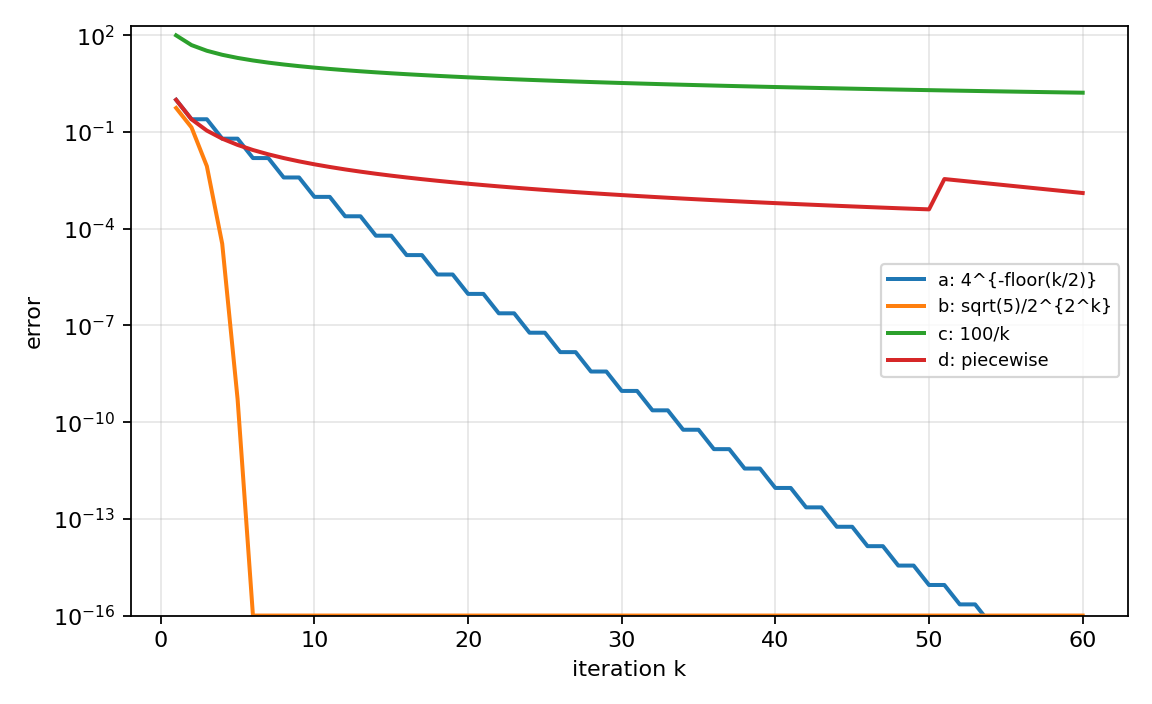
\includegraphics[width=0.78\textwidth]{hw10_2_1_semilogy.png}
\end{center}


\section{梯度下降法}
\paragraph{3.1} 如课件（P16），考虑2维2次函数优化问题:
$$\min_x f(x)=\frac{1}{2}\left(x_1^2+\gamma x_2^2\right)$$
其中，$\gamma \geq 1$。当选取初始点$x^{0}=(\gamma,1)$时，试证明采用精准线搜索时，有下式成立
$$\frac{\|{x_k-x^*}\|_2}{\|{x_0-x^*}\|_2}=
\left(\frac{\gamma-1}{\gamma+1}\right)^k$$

\textbf{证明：}
该二次函数的最优解为
\[
  x^\star=(0,0).
\]
记
\[
  Q=\begin{pmatrix}1&0\\0&\gamma\end{pmatrix},
  \qquad
  f(x)=\frac12x^TQx,\qquad
  \nabla f(x)=Qx.
\]
若 $\gamma=1$，则 $Q=I$，初始点 $x^0=(1,1)$。精准线搜索取
$t_0=1$，于是
\[
  x^1=x^0-\nabla f(x^0)=0=x^\star,
\]
结论显然成立。下面只需考虑 $\gamma>1$。

设
\[
  g^k=\nabla f(x^k)=Qx^k.
\]
精准线搜索是在方向 $-g^k$ 上求解一维最小化问题
\[
  t_k=\arg\min_{t\geq0}\phi_k(t),
  \qquad
  \phi_k(t)=f(x^k-tg^k).
\]
因为
\[
  \phi_k(t)=\frac12(x^k-tg^k)^TQ(x^k-tg^k),
\]
对 $t$ 求导可得
\[
  \phi_k'(t)
  =-(g^k)^TQx^k+t(g^k)^TQg^k.
\]
又由于 $g^k=Qx^k$，有
\[
  (g^k)^TQx^k=(g^k)^Tg^k.
\]
令 $\phi_k'(t)=0$，得到精准线搜索步长
\[
  t_k
  =\frac{(g^k)^Tg^k}{(g^k)^TQg^k}
  =\frac{\nabla f(x^k)^T\nabla f(x^k)}
  {\nabla f(x^k)^TQ\nabla f(x^k)}.
\]
因为 $Q\succ0$ 且 $g^k\neq0$ 时分母为正，所以上式给出的确是该直线上的最小点。

下面证明迭代点具有形式
\[
  x^k=r^k(\gamma,(-1)^k),
  \qquad
  r=\frac{\gamma-1}{\gamma+1}.
\]
当 $k=0$ 时显然成立。若 $x^k=r^k(\gamma,(-1)^k)$，则
\[
  \nabla f(x^k)=r^k(\gamma,\gamma(-1)^k).
\]
于是
\[
  \|\nabla f(x^k)\|_2^2
  =\gamma^2r^{2k}+\gamma^2r^{2k}
  =2\gamma^2r^{2k},
\]
并且
\[
\begin{aligned}
  \nabla f(x^k)^TQ\nabla f(x^k)
  &=(\gamma r^k)^2+\gamma(\gamma(-1)^kr^k)^2\\
  &=\gamma^2r^{2k}+\gamma^3r^{2k}.
\end{aligned}
\]
代入精准线搜索步长公式得到
\[
  t_k=\frac{2\gamma^2r^{2k}}
  {\gamma^2r^{2k}+\gamma^3r^{2k}}
  =\frac{2}{\gamma+1}.
\]
再代入梯度下降迭代
\[
  x^{k+1}=x^k-t_k\nabla f(x^k),
\]
逐分量计算为
\[
\begin{aligned}
  x^{k+1}
  &=x^k-t_k\nabla f(x^k)\\
  &=r^k\left(
    \gamma\left(1-\frac{2}{\gamma+1}\right),
    (-1)^k\left(1-\frac{2\gamma}{\gamma+1}\right)
  \right)\\
  &=r^k\left(
    \gamma\frac{\gamma-1}{\gamma+1},
    (-1)^k\frac{1-\gamma}{\gamma+1}
  \right)\\
  &=r^{k+1}(\gamma,(-1)^{k+1}).
\end{aligned}
\]
归纳成立。因此
\[
  \|x^k-x^\star\|_2
  =r^k\sqrt{\gamma^2+1},
  \qquad
  \|x^0-x^\star\|_2=\sqrt{\gamma^2+1}.
\]
所以
\[
  \frac{\|x_k-x^\star\|_2}{\|x_0-x^\star\|_2}
  =
  \left(\frac{\gamma-1}{\gamma+1}\right)^k.
\]
当 $\gamma=1$ 时，精准线搜索一步到达最优解，上式仍可按 $r=0$ 理解。


\paragraph{3.2} 考虑教材9.3.2中的函数
$$f(x_1, x_2) = e^{x_1+3x_2-0.1} + e^{x_1-3x_2-0.1} + e^{-x_1-0.1}$$
\begin{enumerate}
	\item 最优值$f^*$与最优解$x^*$分别是什么?
	\item 利用回溯线搜索（$\alpha=0.1$, $\beta=0.7$）求解，可设置初始点为$x^0=(0,0)$。请画出$f(x^k)-f^*$随着迭代次数$k$变化的图像（semilogy形式，展示30次迭代就可以）。 
    注意：你可以利用Matlab或Python自行画图，并将相关代码附在作业后面。
\end{enumerate}

\textbf{解：}
令
\[
  a=e^{x_1+3x_2-0.1},\qquad
  b=e^{x_1-3x_2-0.1},\qquad
  c=e^{-x_1-0.1}.
\]
则
\[
  \nabla f(x)=
  \begin{pmatrix}
    a+b-c\\
    3a-3b
  \end{pmatrix}.
\]
在最优点处有 $\nabla f(x^\star)=0$，所以
\[
  a=b,\qquad c=a+b=2a.
\]
由 $a=b$ 得 $x_2^\star=0$。再由 $c=2a$ 得
\[
  e^{-x_1^\star-0.1}=2e^{x_1^\star-0.1},
  \qquad
  e^{-2x_1^\star}=2,
\]
因此
\[
  x_1^\star=-\frac12\log 2.
\]
所以
\[
  \boxed{
  x^\star=\left(-\frac12\log2,\ 0\right).}
\]
由于该函数是若干指数仿射函数之和，且对应方向张成 $\mathbb R^2$，所以 $f$ 严格凸；上述驻点即为全局唯一最优解。最优值为
\[
\begin{aligned}
  f^\star
  &=2e^{-\frac12\log2-0.1}
    +e^{\frac12\log2-0.1}\\
  &=2\sqrt2\,e^{-0.1}.
\end{aligned}
\]
即
\[
  \boxed{f^\star=2\sqrt2\,e^{-0.1}\approx 2.5593.}
\]

回溯线搜索使用 Armijo 条件
\[
  f(x^k-t_k\nabla f(x^k))
  \leq f(x^k)-\alpha t_k\|\nabla f(x^k)\|_2^2,
\]
其中初始步长取 $1$，若不满足则令 $t_k\leftarrow \beta t_k$。取
$\alpha=0.1,\ \beta=0.7,\ x^0=(0,0)$，得到下图。

\begin{center}
  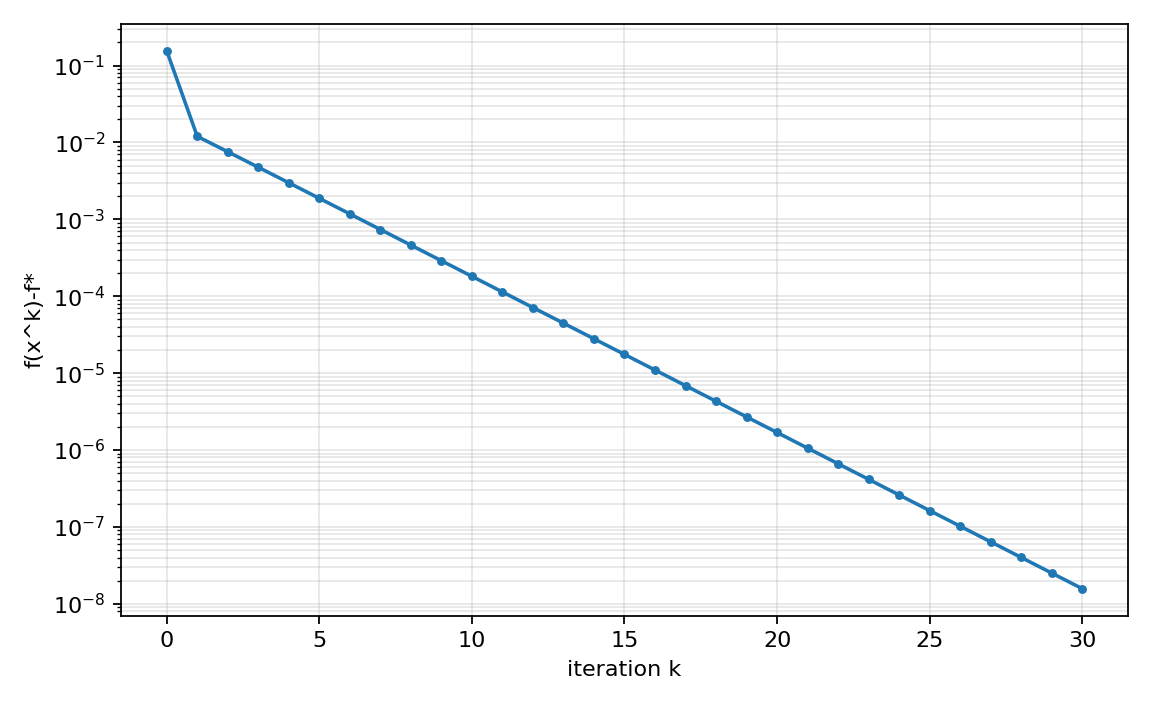
\includegraphics[width=0.78\textwidth]{hw10_3_2_semilogy.png}
\end{center}

数值上第 $30$ 次迭代约为
\[
  x^{30}\approx(-0.34646271,\ 0),
  \qquad
  f(x^{30})-f^\star\approx 1.57\times 10^{-8}.
\]

\paragraph{3.3} 假设函数是$f$是凸的且$L$-光滑，试证明
$$\left(\nabla f(x)-\nabla f(y)\right)^T(x-y) \geq \frac{1}{L} ||\nabla f(x)-\nabla f(y)||_2^2$$

\textbf{证明：}
固定 $y$，定义
\[
  \phi(z)=f(z)-\nabla f(y)^Tz.
\]
则 $\phi$ 仍然是凸函数且 $L$-光滑，并且
\[
  \nabla\phi(y)=\nabla f(y)-\nabla f(y)=0.
\]
因此 $y$ 是 $\phi$ 的全局最小点。

由 $L$-光滑性，对任意 $x$ 有
\[
  \phi\left(x-\frac1L\nabla\phi(x)\right)
  \leq
  \phi(x)-\frac{1}{2L}\|\nabla\phi(x)\|_2^2.
\]
又因为 $y$ 是 $\phi$ 的最小点，所以
\[
  \phi(y)
  \leq
  \phi\left(x-\frac1L\nabla\phi(x)\right).
\]
合并得到
\[
  f(y)-\nabla f(y)^Ty
  \leq
  f(x)-\nabla f(y)^Tx
  -\frac{1}{2L}\|\nabla f(x)-\nabla f(y)\|_2^2.
\]
交换 $x,y$ 同理可得
\[
  f(x)-\nabla f(x)^Tx
  \leq
  f(y)-\nabla f(x)^Ty
  -\frac{1}{2L}\|\nabla f(x)-\nabla f(y)\|_2^2.
\]
两式相加并整理，得到
\[
  \left(\nabla f(x)-\nabla f(y)\right)^T(x-y)
  \geq
  \frac1L\|\nabla f(x)-\nabla f(y)\|_2^2.
\]
证毕。

\paragraph{3.4} 证明课件梯度下降法课件P34中的定理。提示：
\begin{itemize}
	\item[a] 构建$h(x)=f(x)-\frac{\mu}{2}x^Tx$。利用\textbf{3.3}证明如下性质：
    $$(\nabla f(x) -\nabla f(y))^T(x-y) \geq \frac{\mu L}{\mu+L} \|x-y\|_2^2+\frac{1}{\mu+L}\|\nabla f(x) - \nabla f(y)\|^2_2$$
	\item[b] 开始证明定理，可以从下式开始
    $$\|x^{k+1}-x^*\|_2^2=\|(x^k-x^*)-t\nabla f(x)\|_2^2$$
\end{itemize}

\textbf{证明：}
要证明的定理为：若 $f$ 是 $\mu$-强凸且 $L$-光滑函数，并且在
$\mathbb R^n$ 上有下界，梯度下降法
\[
  x^{k+1}=x^k-t\nabla f(x^k)
\]
采用固定步长
\[
  0<t<\frac{2}{\mu+L},
\]
则
\[
  \|x^k-x^\star\|_2^2
  \leq
  \left(1-t\frac{2\mu L}{\mu+L}\right)^k
  \|x^0-x^\star\|_2^2.
\]

先证明提示中的关键不等式。令
\[
  h(x)=f(x)-\frac{\mu}{2}x^Tx.
\]
当 $L=\mu$ 时，$h$ 是 $0$-光滑凸函数，因此 $\nabla h$ 为常向量，
从而 $\nabla f(x)-\nabla f(y)=\mu(x-y)$，下面的关键不等式取等号成立。
下设 $L>\mu$。由于 $f$ 是 $\mu$-强凸且 $L$-光滑，$h$ 是凸函数，并且是 $(L-\mu)$-光滑函数。由 3.3 应用于 $h$，有
\[
  (\nabla h(x)-\nabla h(y))^T(x-y)
  \geq
  \frac{1}{L-\mu}\|\nabla h(x)-\nabla h(y)\|_2^2.
\]
记
\[
  s=x-y,\qquad
  g=\nabla f(x)-\nabla f(y).
\]
因为
\[
  \nabla h(x)-\nabla h(y)=g-\mu s,
\]
所以上式等价于
\[
  (g-\mu s)^Ts
  \geq
  \frac{1}{L-\mu}\|g-\mu s\|_2^2.
\]
两边乘以 $L-\mu$ 并展开：
\[
  (L-\mu)g^Ts-\mu(L-\mu)\|s\|_2^2
  \geq
  \|g\|_2^2-2\mu g^Ts+\mu^2\|s\|_2^2.
\]
整理得
\[
  (\mu+L)g^Ts
  \geq
  \mu L\|s\|_2^2+\|g\|_2^2,
\]
也就是
\[
  (\nabla f(x)-\nabla f(y))^T(x-y)
  \geq
  \frac{\mu L}{\mu+L}\|x-y\|_2^2
  +\frac{1}{\mu+L}
  \|\nabla f(x)-\nabla f(y)\|_2^2.
\]

下面证明收敛结论。由于 $f$ 强凸且有下界，它有唯一最优解 $x^\star$，并满足
\[
  \nabla f(x^\star)=0.
\]
令
\[
  s_k=x^k-x^\star,\qquad
  g_k=\nabla f(x^k)-\nabla f(x^\star)=\nabla f(x^k).
\]
由梯度下降迭代式，
\[
\begin{aligned}
  \|x^{k+1}-x^\star\|_2^2
  &=\|s_k-tg_k\|_2^2\\
  &=\|s_k\|_2^2-2t g_k^Ts_k+t^2\|g_k\|_2^2.
\end{aligned}
\]
将刚刚证明的不等式用于 $x=x^k,\ y=x^\star$，得到
\[
  g_k^Ts_k
  \geq
  \frac{\mu L}{\mu+L}\|s_k\|_2^2
  +\frac{1}{\mu+L}\|g_k\|_2^2.
\]
代入展开式：
\[
\begin{aligned}
  \|x^{k+1}-x^\star\|_2^2
  &\leq
  \left(1-\frac{2t\mu L}{\mu+L}\right)\|s_k\|_2^2
  +\left(t^2-\frac{2t}{\mu+L}\right)\|g_k\|_2^2.
\end{aligned}
\]
因为
\[
  0<t<\frac{2}{\mu+L},
\]
所以
\[
  t^2-\frac{2t}{\mu+L}<0.
\]
舍去这个非正项，有
\[
  \|x^{k+1}-x^\star\|_2^2
  \leq
  \left(1-\frac{2t\mu L}{\mu+L}\right)
  \|x^k-x^\star\|_2^2.
\]
又由 $4\mu L\leq(\mu+L)^2$ 可知该因子非负。递推得到
\[
  \|x^k-x^\star\|_2^2
  \leq
  \left(1-t\frac{2\mu L}{\mu+L}\right)^k
  \|x^0-x^\star\|_2^2.
\]
证毕。


\section{次梯度下降法}
\paragraph{4.1} 证明$\partial f(x)$是凸集合。 

\textbf{证明：}
按照次梯度定义，
\[
  \partial f(x)
  =
  \{g\mid f(y)\geq f(x)+g^T(y-x),\ \forall y\}.
\]
任取
\[
  g_1,g_2\in\partial f(x),\qquad \theta\in[0,1].
\]
则对任意 $y$，有
\[
  f(y)\geq f(x)+g_1^T(y-x),
  \qquad
  f(y)\geq f(x)+g_2^T(y-x).
\]
两式分别乘以 $\theta$ 和 $1-\theta$ 后相加，得到
\[
\begin{aligned}
  f(y)
  &\geq
  f(x)+\left(\theta g_1+(1-\theta)g_2\right)^T(y-x).
\end{aligned}
\]
因此
\[
  \theta g_1+(1-\theta)g_2\in\partial f(x).
\]
这说明 $\partial f(x)$ 对任意凸组合封闭，所以 $\partial f(x)$ 是凸集合。

\section*{附录：作图代码}

\IfFileExists{generate_figures.py}{
  \lstinputlisting[language=Python]{generate_figures.py}
}{
  \lstinputlisting[language=Python]{hw10/generate_figures.py}
}


\end{document}
